\documentclass[12pt, letterpaper]{article}
\usepackage{amsmath}
\usepackage{amssymb}
\usepackage{tikz}
\usepackage[utf8]{inputenc}
\usetikzlibrary{patterns,arrows,decorations.pathreplacing}
\usepackage{xcolor}
\usetikzlibrary{patterns}

\begin{document}

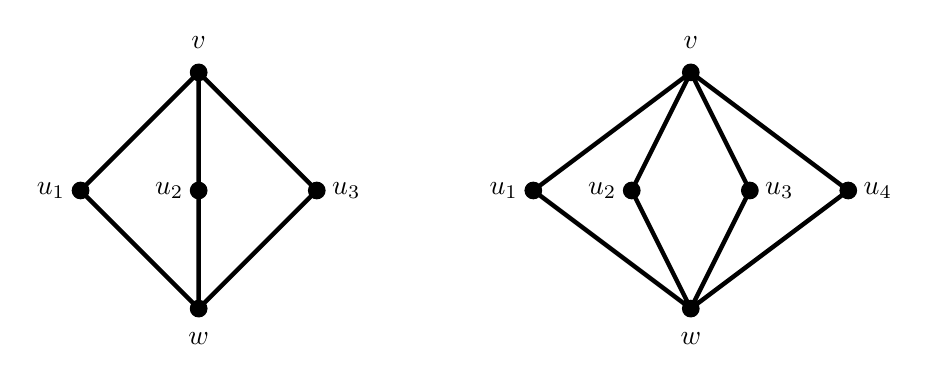
\begin{tikzpicture}[scale=0.25]
\draw[ultra thick](0,-6)--(0,0)(0,-6)--(6,0)(0,-6)--(-6,0)(0,6)--(6,0)(0,6)--(-6,0)(0,6)--(0,0);
\draw[fill=black] (0,-6) circle (12pt);
\draw[fill=black] (0,6) circle (12pt);
\draw[fill=black] (0,0) circle (12pt);
\draw[fill=black] (6,0) circle (12pt);
\draw[fill=black] (-6,0) circle (12pt);
\node at (0,-7.5) {$w$};
\node at (0,7.5) {$v$};
\node at (-7.5,0) {$u_1$};
\node at (-1.5,0) {$u_2$};
\node at (7.5,0) {$u_3$};

\begin{scope}[shift={(25,0)}]
\draw[ultra thick](0,-6)--(3,0)(0,-6)--(8,0)(0,-6)--(-3,0)(0,-6)--(-8,0)(0,6)--(3,0)(0,6)--(8,0)(0,6)--(-3,0)(0,6)--(-8,0);
\draw[fill=black] (0,-6) circle (12pt);
\draw[fill=black] (0,6) circle (12pt);
\draw[fill=black] (3,0) circle (12pt);
\draw[fill=black] (8,0) circle (12pt);
\draw[fill=black] (-3,0) circle (12pt);
\draw[fill=black] (-8,0) circle (12pt);
\node at (0,-7.5) {$w$};
\node at (0,7.5) {$v$};
\node at (-9.5,0) {$u_1$};
\node at (-4.5,0) {$u_2$};
\node at (9.5,0) {$u_4$};
\node at (4.5,0) {$u_3$};
\end{scope}
\end{tikzpicture}

\end{document}